\documentclass[aspectratio=169,11pt]{beamer}
\usepackage{ctex}
\usepackage{graphicx}
\usepackage{booktabs}
\usepackage{tikz}
\usepackage{pgfplots}
\usepackage{amsmath}
\usepackage{fontawesome5}
\usepackage{algorithm}
\usepackage{algorithmic}
\usepackage{colortbl}

\pgfplotsset{compat=1.18}
\usetikzlibrary{shapes,arrows,positioning,shadows,calc}

% 主题设置
\usetheme{Madrid}
\usecolortheme{whale}
\setbeamertemplate{navigation symbols}{}
\setbeamertemplate{footline}[frame number]

% 自定义颜色
\definecolor{primary}{RGB}{0, 83, 156}
\definecolor{secondary}{RGB}{0, 150, 136}
\definecolor{accent}{RGB}{255, 152, 0}
\definecolor{successgreen}{RGB}{34, 139, 34}
\definecolor{dangerred}{RGB}{220, 20, 60}
\definecolor{codeblue}{RGB}{41, 128, 185}
\definecolor{codebg}{RGB}{248, 248, 248}

\setbeamercolor{title}{fg=white,bg=primary}
\setbeamercolor{frametitle}{fg=white,bg=primary}
\setbeamercolor{block title}{fg=white,bg=secondary}

% 图片路径 - 使用 PDF 矢量图
\graphicspath{{figures/}}

% 文档信息
\title[Casevo 智能体决策优化]{基于 Casevo 框架的智能体决策能力优化研究}
\subtitle{Tree of Thought 在社会模拟中的应用与评估}
\author{王宇东(组长)、陈文远}
\institute{人工智能与社会课程}
\date{2025年12月}

\begin{document}

%==============================================================================
% 标题页
%==============================================================================
\begin{frame}
\titlepage
\end{frame}

%==============================================================================
% 目录
%==============================================================================
\begin{frame}{报告大纲}
\tableofcontents
\end{frame}

%==============================================================================
\section{研究背景}
%==============================================================================

\begin{frame}{研究动机}
\begin{columns}
\begin{column}{0.55\textwidth}
\textbf{Casevo 框架}
\begin{itemize}
    \item 基于 LLM 的多智能体社会模拟框架
    \item 支持选举投票、资源分配、信息传播等场景
    \item 集成 CoT 推理、RAG 记忆、反思机制
\end{itemize}

\vspace{0.5cm}
\textbf{存在的问题}
\begin{itemize}
    \item 线性 CoT 在复杂决策中波动大
    \item 记忆检索效率和准确性有限
    \item 多智能体协同机制不完善
\end{itemize}
\end{column}
\begin{column}{0.42\textwidth}
\centering
% 使用 TikZ 绘制小世界网络拓扑
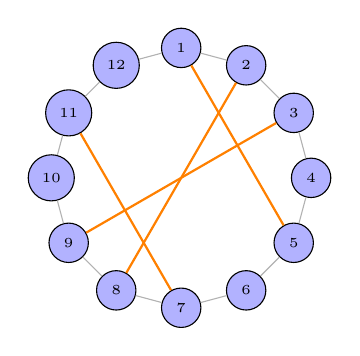
\begin{tikzpicture}[scale=0.75]
    \def\n{12}
    \def\r{2.2}
    % 绘制节点(圆形排列)
    \foreach \i in {1,...,\n} {
        \pgfmathsetmacro{\angle}{90 - (\i-1)*360/\n}
        \node[circle, draw, fill=blue!30, minimum size=0.5cm, font=\tiny] (n\i) at (\angle:\r) {\i};
    }
    % 绘制邻近连接(小世界网络)
    \foreach \i in {1,...,\n} {
        \pgfmathtruncatemacro{\next}{mod(\i, \n) + 1}
        \draw[gray!60] (n\i) -- (n\next);
    }
    % 绘制跳跃连接(长程连接)
    \draw[orange, thick] (n1) -- (n5);
    \draw[orange, thick] (n3) -- (n9);
    \draw[orange, thick] (n7) -- (n11);
    \draw[orange, thick] (n2) -- (n8);
\end{tikzpicture}

\vspace{0.2cm}
\small 小世界网络拓扑
\end{column}
\end{columns}
\end{frame}

%==============================================================================
\section{研究方法}
%==============================================================================

\begin{frame}{四项优化策略概览}
\centering
\begin{tikzpicture}[
    box/.style={draw, rounded corners=8pt, minimum width=5.5cm, minimum height=1.8cm, align=center, font=\small, line width=1.2pt, drop shadow},
    arrow/.style={->, thick, >=stealth, line width=1.5pt}
]
    % 中心节点
    \node[draw, circle, fill=primary!30, minimum size=2cm, line width=2pt, font=\large\bfseries] (center) at (0,0) {决策优化};
    
    % 四个策略
    \node[box, fill=blue!15] (tot) at (-5,2) {\textbf{1. Tree of Thought}\\多路径推理 + 剪枝};
    \node[box, fill=green!15] (mem) at (5,2) {\textbf{2. 增强记忆检索}\\时间衰减 + 情境匹配};
    \node[box, fill=orange!15] (ref) at (-5,-2) {\textbf{3. 动态反思机制}\\置信度触发自我反思};
    \node[box, fill=purple!15] (col) at (5,-2) {\textbf{4. 协同决策}\\多智能体信息交换};
    
    % 连线
    \draw[arrow, blue!60] (tot) -- (center);
    \draw[arrow, green!60] (mem) -- (center);
    \draw[arrow, orange!60] (ref) -- (center);
    \draw[arrow, purple!60] (col) -- (center);
\end{tikzpicture}
\end{frame}

\begin{frame}{策略1:Tree of Thought 实现}
\begin{columns}
\begin{column}{0.48\textwidth}
\textbf{核心思想}:将线性推理扩展为树状探索

\vspace{0.3cm}
\textbf{实现细节}:
\begin{enumerate}
    \item \textbf{分支生成}:LLM 生成多个候选推理路径
    \item \textbf{分支评估}:LLM 对每个路径打分 (0-1)
    \item \textbf{Beam Search}:保留 Top-K 高分路径
    \item \textbf{剪枝}:丢弃低于阈值 $\theta$ 的路径
    \item \textbf{迭代}:重复直到达到最大深度
\end{enumerate}

\vspace{0.3cm}
\textbf{关键参数}:
\begin{itemize}
    \item 最大深度 $D = 3$
    \item 束宽度 $K = 3$
    \item 剪枝阈值 $\theta = 0.6$
\end{itemize}
\end{column}
\begin{column}{0.5\textwidth}
\centering
\begin{tikzpicture}[
    level 1/.style={sibling distance=2.8cm, level distance=1.5cm},
    level 2/.style={sibling distance=1.4cm, level distance=1.5cm},
    node/.style={circle, draw, minimum size=0.6cm, font=\scriptsize, line width=0.8pt}
]
    \node[node, fill=blue!30] (root) {问题}
        child {node[node, fill=green!30] {0.8}
            child {node[node, fill=green!40] {\textbf{0.9}}}
            child {node[node, fill=gray!30, dashed] {0.4}}
        }
        child {node[node, fill=green!30] {0.7}
            child {node[node, fill=gray!30, dashed] {0.5}}
            child {node[node, fill=green!30] {0.7}}
        }
        child {node[node, fill=gray!30, dashed] {0.3}
        };
    
    \node[right of=root, xshift=3.5cm, yshift=-0.5cm, font=\scriptsize, align=left] {
        \textcolor{green!60!black}{$\bullet$ 保留路径}\\
        \textcolor{gray}{$\circ$ 剪枝路径}
    };
\end{tikzpicture}

\vspace{0.3cm}
\small\textbf{每层}:生成 $\to$ 评估 $\to$ 保留 Top-K
\end{column}
\end{columns}
\end{frame}

\begin{frame}{策略1:ToT 伪代码}
\begin{columns}
\begin{column}{0.52\textwidth}
\begin{block}{ToT 推理算法}
\scriptsize
\textbf{输入}:问题$P$, 深度$D$, 束宽$K$, 阈值$\theta$ \quad \textbf{输出}:$d^*$

\vspace{0.1cm}
\begin{tabular}{@{}r@{\;}l@{}}
1. & $\mathcal{B}_0 \leftarrow \{(\text{root}, 1.0)\}$ \\
2. & \textbf{for} $d = 1$ \textbf{to} $D$: \\
3. & \quad $\mathcal{C} \leftarrow \emptyset$ \\
4. & \quad \textbf{for} $(n, s) \in \mathcal{B}_{d-1}$: \\
5. & \quad\quad $B \leftarrow \text{LLM\_Gen}(n, P)$ \\
6. & \quad\quad \textbf{for} $b \in B$: \\
7. & \quad\quad\quad $s_b \leftarrow \text{LLM\_Eval}(b)$ \\
8. & \quad\quad\quad \textbf{if} $s_b \geq \theta$: $\mathcal{C} \cup= \{(b, s_b)\}$ \\
9. & \quad $\mathcal{B}_d \leftarrow \text{TopK}(\mathcal{C}, K)$ \\
10. & \textbf{return} $\arg\max \mathcal{B}_D$ \\
\end{tabular}
\end{block}
\end{column}
\begin{column}{0.45\textwidth}
\begin{alertblock}{关键点}
\small
\begin{itemize}
    \item 每次 LLM 调用都有成本
    \item 深度$D$和分支数决定调用次数
    \item 阈值$\theta$控制探索广度
\end{itemize}
\end{alertblock}

\vspace{0.2cm}
\begin{exampleblock}{LLM 调用次数}
\centering
$O(K \times B \times D)$\\
\scriptsize $K$=束宽,$B$=分支数,$D$=深度
\end{exampleblock}
\end{column}
\end{columns}
\end{frame}

\begin{frame}{策略2:增强记忆检索}
\begin{columns}
\begin{column}{0.5\textwidth}
\textbf{问题}:原始 RAG 仅用语义相似度

\vspace{0.2cm}
\textbf{改进}:多因素加权检索
\begin{equation*}
score(m) = sim(q, m) \cdot w_t \cdot w_c
\end{equation*}

\small
\begin{itemize}
    \item $sim(q, m)$:语义相似度
    \item $w_t = e^{-\lambda \cdot \Delta t}$:\textcolor{blue}{时间衰减}
    \item $w_c$:\textcolor{green!60!black}{情境匹配度}
\end{itemize}

\vspace{0.15cm}
\textbf{实现步骤}:嵌入 $\to$ 相似度 $\to$ 时间衰减($\lambda$=0.1) $\to$ 情境匹配 $\to$ Top-K
\end{column}
\begin{column}{0.48\textwidth}
\centering
\begin{tikzpicture}[scale=0.85]
    \begin{axis}[
        width=6cm, height=4.2cm,
        xlabel={时间差 $\Delta t$},
        ylabel={$w_t$},
        xmin=0, xmax=50,
        ymin=0, ymax=1.1,
        grid=major,
        font=\small
    ]
    \addplot[blue, thick, domain=0:50, samples=100] {exp(-0.1*x)};
    \addplot[only marks, mark=*, red] coordinates {(0, 1) (10, 0.368) (20, 0.135) (30, 0.05)};
    \end{axis}
\end{tikzpicture}

\vspace{0.1cm}
\small $w_t = e^{-0.1 \cdot \Delta t}$,近期记忆权重更高
\end{column}
\end{columns}
\end{frame}

\begin{frame}{策略3-4:动态反思 \& 协同决策}
\begin{columns}
\begin{column}{0.48\textwidth}
\textbf{3. 动态反思机制}

\vspace{0.3cm}
\centering
\begin{tikzpicture}[scale=0.85,
    box/.style={draw, rounded corners, minimum width=2.2cm, minimum height=0.55cm, align=center, font=\scriptsize},
    arrow/.style={->, thick, >=stealth}
]
    \node[box, fill=blue!25] (dec) at (0,0) {初始决策};
    \node[box, fill=orange!25] (conf) at (0,-1.2) {置信度评估};
    \node[box, fill=red!25] (ref) at (3.2,-1.2) {深度反思};
    \node[box, fill=green!25] (out) at (0,-2.4) {最终决策};
    
    \draw[arrow] (dec) -- (conf);
    \draw[arrow] (conf.east) -- node[above, font=\tiny] {$c<0.6$} (ref.west);
    % 返回箭头:从深度反思下方绕回
    \draw[arrow] (ref.south) -- ++(0,-0.35) -| node[pos=0.25, below, font=\tiny] {重评估} (conf.south);
    \draw[arrow] (conf.west) -- ++(-0.5,0) |- node[pos=0.2, left, font=\tiny] {$c \geq 0.6$} (out.west);
\end{tikzpicture}

\vspace{0.15cm}
\footnotesize 置信度低于阈值时触发反思
\end{column}
\begin{column}{0.48\textwidth}
\textbf{4. 协同决策}

\vspace{0.3cm}
\centering
\begin{tikzpicture}[scale=0.9,
    agent/.style={draw, circle, minimum size=0.9cm, font=\small, line width=1pt},
    arrow/.style={<->, thick, gray!70, >=stealth}
]
    \node[agent, fill=blue!25] (a1) at (0,0) {$A_1$};
    \node[agent, fill=green!25] (a2) at (2.2,0) {$A_2$};
    \node[agent, fill=orange!25] (a3) at (1.1,-1.6) {$A_3$};
    
    \draw[arrow] (a1) -- node[above, font=\tiny] {观点交换} (a2);
    \draw[arrow] (a1) -- node[left, font=\tiny] {协商} (a3);
    \draw[arrow] (a2) -- node[right, font=\tiny] {调整} (a3);
\end{tikzpicture}

\vspace{0.2cm}
\footnotesize 智能体间迭代协商达成共识
\end{column}
\end{columns}

\vspace{0.4cm}
\begin{center}
\begin{tikzpicture}
\node[draw, rounded corners, fill=accent!15, inner sep=6pt, font=\footnotesize] {
    \textbf{注}:实验结果显示,动态反思和协同决策的效果有限,详见后续分析
};
\end{tikzpicture}
\end{center}
\end{frame}

\begin{frame}{实验设计}
\begin{table}
\centering
\begin{tabular}{lccc}
\toprule
\textbf{场景} & \textbf{Agent数} & \textbf{轮数} & \textbf{核心挑战} \\
\midrule
选举投票 & 30 & 6 & 社会影响下的态度演化 \\
资源分配 & 20 & $\leq$5 & 快速收敛到公平分配 \\
信息传播 & 50 & 10 & 阻止虚假信息扩散 \\
\bottomrule
\end{tabular}
\end{table}

\vspace{0.3cm}
\begin{center}
\begin{tikzpicture}
\node[draw, rounded corners, fill=primary!10, inner sep=10pt] {
    \textbf{实验规模}: 5 组配置 $\times$ 3 次运行 $\times$ 3 场景 = \textcolor{primary}{\textbf{45 次实验}}
};
\end{tikzpicture}
\end{center}

\vspace{0.3cm}
\textbf{五组实验配置}:
\begin{itemize}
    \item \texttt{baseline\_cot}:原始 CoT
    \item \texttt{tot\_only}:仅启用 ToT
    \item \texttt{tot+memory}:ToT + 增强记忆
    \item \texttt{tot+reflection}:ToT + 动态反思
    \item \texttt{full}:全部启用
\end{itemize}
\end{frame}

%==============================================================================
\section{实验结果}
%==============================================================================

\begin{frame}{核心发现:ToT 效果总览}
\centering
\includegraphics[width=0.85\textwidth]{fig_tot_vs_cot.pdf}

\vspace{0.3cm}
\begin{columns}
\begin{column}{0.32\textwidth}
\centering
\textcolor{successgreen}{\faCheckCircle} 资源分配\\
\textbf{+13.6\%}
\end{column}
\begin{column}{0.32\textwidth}
\centering
\textcolor{successgreen}{\faCheckCircle} 信息传播\\
\textbf{+10.6\%}
\end{column}
\begin{column}{0.32\textwidth}
\centering
\textcolor{dangerred}{\faTimesCircle} 选举投票\\
\textbf{-17.0\%}
\end{column}
\end{columns}

\vspace{0.3cm}
\begin{alertblock}{关键发现}
ToT 具有\textbf{场景敏感性}——多路径推理并非在所有场景都能带来收益!
\end{alertblock}
\end{frame}

\begin{frame}{选举投票场景:推理能力 vs 综合得分}
\begin{columns}
\begin{column}{0.48\textwidth}
\begin{table}
\small
\begin{tabular}{lcc}
\toprule
\textbf{指标} & \textbf{CoT} & \textbf{ToT} \\
\midrule
推理能力得分 & 0.43 & \textcolor{successgreen}{\textbf{0.95}} \\
综合得分 & \textcolor{successgreen}{\textbf{0.609}} & 0.505 \\
推理深度 & 2 & 5 \\
分支探索数 & 1 & 40 \\
连贯性分数 & 0.41 & 0.82 \\
\bottomrule
\end{tabular}
\end{table}

\vspace{0.3cm}
\begin{block}{矛盾现象}
\begin{itemize}
    \item 推理能力 \textcolor{successgreen}{+121\%}
    \item 综合得分 \textcolor{dangerred}{-17\%}
\end{itemize}
\end{block}
\end{column}
\begin{column}{0.5\textwidth}
\centering
\includegraphics[width=\textwidth]{fig_election_evolution.pdf}
\small 选民态度演化对比
\end{column}
\end{columns}
\end{frame}

\begin{frame}{资源分配场景:ToT + 记忆最优}
\begin{columns}
\begin{column}{0.48\textwidth}
\begin{table}
\small
\begin{tabular}{lcc}
\toprule
\textbf{配置} & \textbf{收敛轮数} & \textbf{标准差} \\
\midrule
baseline\_cot & 3.00 & 0.00 \\
tot\_only & 2.33 & 0.58 \\
\rowcolor{green!20} \textbf{tot+memory} & \textbf{2.00} & \textbf{0.00} \\
tot+reflection & 3.00 & 1.00 \\
full & 2.33 & 0.58 \\
\bottomrule
\end{tabular}
\end{table}

\vspace{0.3cm}
\begin{exampleblock}{最优配置}
\textbf{ToT + 增强记忆}:收敛最快(2轮)、稳定性最高($\sigma=0$)
\end{exampleblock}
\end{column}
\begin{column}{0.5\textwidth}
\centering
\includegraphics[width=\textwidth]{fig_resource_convergence.pdf}
\small 资源分配收敛分析
\end{column}
\end{columns}
\end{frame}

\begin{frame}{信息传播场景:ToT 的过度保守行为}
\centering
\includegraphics[width=0.75\textwidth]{fig_info_spread.pdf}

\vspace{0.3cm}
\begin{columns}
\begin{column}{0.48\textwidth}
\begin{table}
\small
\begin{tabular}{lcc}
\toprule
\textbf{指标} & \textbf{CoT} & \textbf{ToT} \\
\midrule
虚假信任率 & 11.6\% & \textcolor{successgreen}{\textbf{0\%}} \\
整体准确率 & \textbf{60.7\%} & \textcolor{dangerred}{50.7\%} \\
信息传播数 & 7 & \textcolor{dangerred}{\textbf{0}} \\
\bottomrule
\end{tabular}
\end{table}
\end{column}
\begin{column}{0.48\textwidth}
\begin{alertblock}{过度保守}
ToT 不仅阻止了虚假信息,\\也阻止了\textbf{所有真实信息}的传播!\\
\small "宁可错杀一千,不可放过一个"
\end{alertblock}
\end{column}
\end{columns}
\end{frame}

%==============================================================================
\section{综合分析}
%==============================================================================

\begin{frame}{组件贡献度分析}
\centering
\includegraphics[width=0.85\textwidth]{fig_component_contribution.pdf}

\vspace{0.3cm}
\begin{columns}
\begin{column}{0.32\textwidth}
\centering
\textcolor{successgreen}{\faStar\faStar\faStar\faStar\faStar}\\
\textbf{ToT}\\
核心贡献者
\end{column}
\begin{column}{0.32\textwidth}
\centering
\textcolor{accent}{\faStar\faStar\faStar}\\
\textbf{增强记忆}\\
场景依赖
\end{column}
\begin{column}{0.32\textwidth}
\centering
\textcolor{dangerred}{\faStar}\\
\textbf{反思/协同}\\
效果有限
\end{column}
\end{columns}
\end{frame}

\begin{frame}{消融实验:组件叠加效应}
\begin{columns}
\begin{column}{0.48\textwidth}
\centering
\includegraphics[width=\textwidth]{fig_ablation_comparison.pdf}
\end{column}
\begin{column}{0.48\textwidth}
\begin{table}
\small
\begin{tabular}{lcc}
\toprule
\textbf{场景} & \textbf{tot\_only} & \textbf{full} \\
\midrule
选举投票 & 0.505 & 0.504 \\
资源分配 & 2.33轮 & 2.33轮 \\
信息传播 & 50.7\% & 50.7\% \\
\bottomrule
\end{tabular}
\end{table}

\vspace{0.5cm}
\begin{alertblock}{意外发现}
\centering
组件叠加无协同效应\\
\Large $1 + 1 \leq 2$
\end{alertblock}
\end{column}
\end{columns}
\end{frame}

\begin{frame}{ToT 的场景行为模式}
\centering
\begin{tikzpicture}[
    box/.style={draw, rounded corners=6pt, minimum width=3cm, minimum height=2cm, align=center, font=\small, line width=1pt},
    arrow/.style={->, thick, >=stealth, line width=1.2pt},
    effect/.style={font=\small\bfseries, fill=white, rounded corners=2pt, inner sep=2pt}
]
    \node[draw, circle, fill=red!30, minimum size=1.6cm, line width=1.5pt, font=\large\bfseries] (tot) at (0,2.5) {ToT};
    
    \node[box, fill=blue!25, drop shadow] (nego) at (-4.5,0) {
        \textbf{协商类}\\[0.1em]
        \textcolor{gray}{(资源分配)}\\[0.2em]
        更聪明的协商\\
        更快收敛
    };
    \node[box, fill=orange!25, drop shadow] (judge) at (0,0) {
        \textbf{判断类}\\[0.1em]
        \textcolor{gray}{(信息传播)}\\[0.2em]
        过度谨慎\\
        拒绝所有信息
    };
    \node[box, fill=green!25, drop shadow] (attitude) at (4.5,0) {
        \textbf{态度类}\\[0.1em]
        \textcolor{gray}{(选举投票)}\\[0.2em]
        更深入推理\\
        更多不确定性
    };
    
    \draw[arrow, blue!60] (tot) -- (nego);
    \draw[arrow, orange!60] (tot) -- (judge);
    \draw[arrow, green!60] (tot) -- (attitude);
    
    \node[effect, text=successgreen] at (-2.8,1.5) {\textbf{+33\%}};
    \node[effect, text=accent] at (0.5,1.5) {\textbf{±0\%}};
    \node[effect, text=successgreen] at (2.8,1.5) {\textbf{+121\%}};
\end{tikzpicture}
\end{frame}

%==============================================================================
\section{成本效益分析}
%==============================================================================

\begin{frame}{计算成本对比}
\begin{columns}
\begin{column}{0.48\textwidth}
\begin{table}
\begin{tabular}{lcc}
\toprule
\textbf{场景} & \textbf{CoT} & \textbf{ToT} \\
\midrule
选举投票 & 3.3s & 747s (\textcolor{dangerred}{\textbf{227×}}) \\
资源分配 & 2.6s & 155s (60×) \\
信息传播 & 1.9s & 152s (80×) \\
\bottomrule
\end{tabular}
\end{table}

\vspace{0.5cm}
\begin{block}{成本来源}
\begin{itemize}
    \item ToT 需要多次 LLM 调用
    \item 分支生成 + 分支评估
    \item 深度越大,成本越高
\end{itemize}
\end{block}
\end{column}
\begin{column}{0.5\textwidth}
\centering
\includegraphics[width=\textwidth]{fig_computational_efficiency.pdf}
\small 各配置响应时间对比
\end{column}
\end{columns}
\end{frame}

\begin{frame}{配置推荐}
\begin{table}
\centering
\begin{tabular}{lcccc}
\toprule
\textbf{场景} & \textbf{baseline} & \textbf{tot\_only} & \textbf{tot+memory} & \textbf{full} \\
\midrule
选举投票 & $\circ$ & $\checkmark$ & $\checkmark\checkmark$ & $\circ$ \\
资源分配 & $\circ$ & $\checkmark$ & $\checkmark\checkmark$ & $\circ$ \\
信息传播 & $\checkmark$ & $\triangle$ & $\triangle$ & $\triangle$ \\
\bottomrule
\end{tabular}
\end{table}

\vspace{0.3cm}
\small $\checkmark\checkmark$: 强烈推荐 \quad $\checkmark$: 推荐 \quad $\circ$: 可用 \quad $\triangle$: 谨慎使用

\vspace{0.5cm}
\begin{center}
\begin{tikzpicture}
\node[draw, rounded corners, fill=successgreen!20, inner sep=12pt, font=\large] {
    \textbf{推荐默认配置}: \texttt{tot\_memory} — 效果最优、成本适中
};
\end{tikzpicture}
\end{center}
\end{frame}

%==============================================================================
\section{结论与展望}
%==============================================================================

\begin{frame}{核心结论}
\begin{columns}
\begin{column}{0.48\textwidth}
\textbf{\textcolor{successgreen}{\faCheckCircle} 验证成功}
\begin{itemize}
    \item ToT 提升推理深度 \textbf{+150\%}
    \item ToT 提升推理连贯性 \textbf{+100\%}
    \item 增强记忆加速协商收敛 \textbf{+33\%}
\end{itemize}

\vspace{0.5cm}
\textbf{\textcolor{dangerred}{\faTimesCircle} 未验证}
\begin{itemize}
    \item 动态反思提升决策质量
    \item 协同决策改善社会效应
    \item 组件叠加产生协同效应
\end{itemize}
\end{column}
\begin{column}{0.48\textwidth}
\textbf{\textcolor{accent}{\faExclamationTriangle} 意外发现}
\begin{itemize}
    \item ToT 在判断类任务中\textbf{过度保守}
    \item 动态反思引入\textbf{不稳定性}
    \item ToT 具有\textbf{场景敏感性}
\end{itemize}

\vspace{0.5cm}
\begin{exampleblock}{核心贡献}
揭示了 ToT 的场景敏感性和过度保守行为,为后续研究提供实证依据
\end{exampleblock}
\end{column}
\end{columns}
\end{frame}

\begin{frame}{研究局限性与未来工作}
\begin{columns}
\begin{column}{0.48\textwidth}
\textbf{研究局限性}
\begin{itemize}
    \item 每组仅 3 次运行,统计显著性有限
    \item Agent 数量有限 (30/20/50)
    \item 依赖特定 LLM 模型版本
    \item 仅测试三种场景类型
\end{itemize}

\vspace{0.5cm}
\textbf{未来工作}
\begin{itemize}
    \item 自适应 ToT:动态调整深度
    \item 置信度校准:避免过度保守
    \item 并行化优化:降低计算成本
    \item 更多场景验证
\end{itemize}
\end{column}
\begin{column}{0.48\textwidth}
\centering
\begin{tikzpicture}[scale=0.8]
    % 改进方向图
    \node[draw, circle, fill=primary!30, minimum size=1.5cm, font=\small\bfseries] (center) at (0,0) {ToT 2.0};
    
    \node[draw, rounded corners, fill=blue!15, font=\scriptsize, align=center] (a1) at (-2.5,1.5) {自适应\\深度};
    \node[draw, rounded corners, fill=green!15, font=\scriptsize, align=center] (a2) at (2.5,1.5) {置信度\\校准};
    \node[draw, rounded corners, fill=orange!15, font=\scriptsize, align=center] (a3) at (-2.5,-1.5) {并行化\\计算};
    \node[draw, rounded corners, fill=purple!15, font=\scriptsize, align=center] (a4) at (2.5,-1.5) {场景\\感知};
    
    \draw[->, thick] (a1) -- (center);
    \draw[->, thick] (a2) -- (center);
    \draw[->, thick] (a3) -- (center);
    \draw[->, thick] (a4) -- (center);
\end{tikzpicture}
\end{column}
\end{columns}
\end{frame}

\begin{frame}{总结}
\centering
\vspace{0.5cm}

\begin{tikzpicture}
\node[draw, rounded corners=10pt, fill=primary!10, inner sep=15pt, text width=12cm, align=center] {
    \Large\textbf{Tree of Thought 是最有效的单一优化策略}\\[0.5cm]
    \normalsize
    在资源分配和信息传播场景显著提升决策质量\\[0.3cm]
    但需注意其\textbf{场景敏感性}和\textbf{过度保守行为}\\[0.5cm]
    \textbf{推荐配置}: \texttt{tot\_memory}
};
\end{tikzpicture}

\vspace{1cm}

\Large\textbf{谢谢!欢迎提问}

\vspace{0.5cm}
\normalsize
\faGithub\ 代码仓库:\texttt{github.com/xxx/casevo-optimization}
\end{frame}

\end{document}
